\subsubsection{JWT-callback и обновление токенов}
Для передачи и обновления JWT в сессии используется callback \textit{jwt}, принимающий параметр \textit{trigger}, позволяющий определить сценарий обработки. Логика работы примерно следующая: при первом входе пользователя (\textit{trigger = signIn}) в токен записываются поля \textit{access\_token}, \textit{refresh\_token} и прочие метаданные; при последующих запросах проверяется срок жизни \textit{access\_token}, и при необходимости инициируется процесс его обновления (\textit{trigger = update}). Если же токен ещё валиден, возвращается неизменённая структура. Пример реализации приведён в листинге~\ref{lst:jwt-callback}.

\begin{lstlisting}[caption={JWT-callback с учётом trigger}, label={lst:jwt-callback}]
	async jwt({ token, trigger, user, session }): Promise<JWT> {
		// Срабатывает при первичной аутентификации (signIn)
		if (trigger === 'signIn') {
			return { ...user, error: null };
		}
		// Если токена ещё нет (например, при восстановлении сессии из куки)
		if (token == null) {
			return { ...session?.user, error: 'another' } as JWT;
		}
		// При запросе обновления (trigger = 'update')
		if (trigger === 'update') {
			return await refreshingProcess(token);
		}
		// Во всех остальных случаях (токен валиден), возвращаем прежнее состояние
		return { ...token, error: null };
	},
\end{lstlisting}

Ниже на рисунке~\ref{fig:auth-refresh} показана вся последовательная диаграмма, иллюстрирующая проверку срока жизни JWT на клиенте и, при необходимости, получение нового токена по refresh-токену. Эта схема помогает понять, как именно Auth.js (или NextAuth.js) взаимодействует с бэкендом для устойчивого хранения и своевременного обновления токенов без лишних повторных запросов.

\begin{figure}[h]
    \centering
    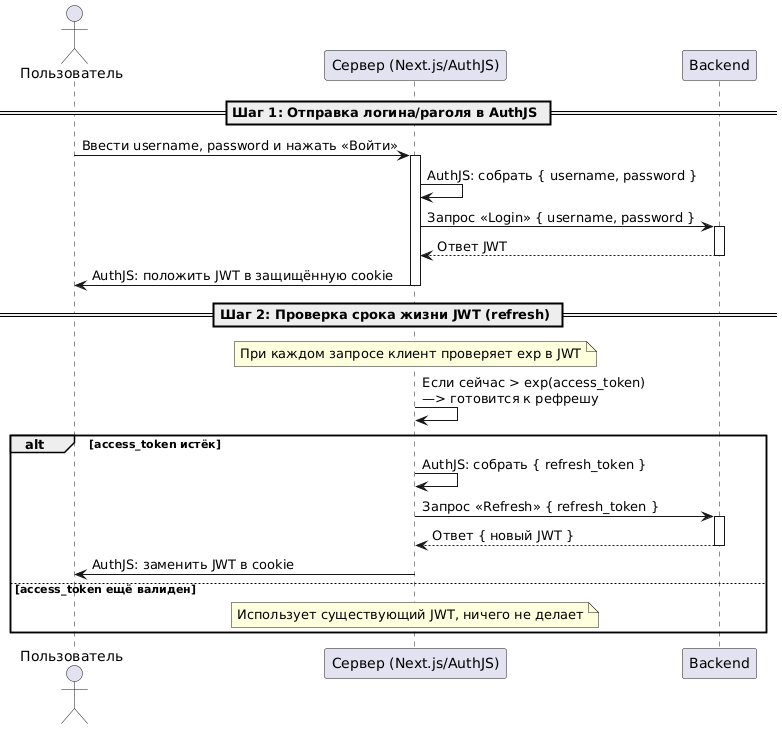
\includegraphics[width=0.9\textwidth]{static/diagrams/AuthRefresh.png}
    \caption{Схема процесса проверки и обновления JWT через refresh-токен}
    \label{fig:auth-refresh}
\end{figure}

На рисунке~\ref{fig:auth-refresh} можно выделить два основных этапа:
\begin{enumerate}
    \item Первичный вход:
    \begin{itemize}
        \item пользователь вводит \textit{username} и \textit{password} в приложение,
        \item Auth.js формирует объект с учётными данными и отправляет запрос на бэкенд (метод \textit{login}),
        \item бэкенд возвращает пару токенов: \textit{access\_token} и \textit{refresh\_token},
        \item Auth.js сохраняет полученный JWT в защищённую cookie или в хранилище клиента.
    \end{itemize}
    \item Проверка срока жизни токена и его обновление:
    \begin{itemize}
        \item при каждом запросе клиент проверяет поле \textit{exp} (срок жизни) в \textit{access\_token},
        \item если текущий момент времени превысил \textit{exp(access\_token)}, начинается подготовка к рефрешу,
        \item в блоке \textit{alt} (альтернативный сценарий) на диаграмме показано, что в случае истёкшего access-токена:
        \begin{itemize}
            \item Auth.js собирает объект с \textit{refresh\_token},
            \item отправляется запрос «Refresh» на бэкенд, передаётся \textit{refresh\_token},
            \item бэкенд возвращает новый \textit{access\_token} и, при необходимости, обновлённый \textit{refresh\_token},
            \item Auth.js заменяет старый JWT в cookie на новый.
        \end{itemize}
        \item если же \textit{access\_token} ещё валиден, Auth.js просто использует существующий токен и не делает дополнительных запросов (промежуточные уведомления внизу диаграммы).
    \end{itemize}
\end{enumerate}

Таким образом, схема на рисунке~\ref{fig:auth-refresh} демонстрирует, что клиент всегда сначала пробует воспользоваться существующим \textit{access\_token}, проверяя его валидность. Только если проверка не проходит, выполняется последовательность обновления, благодаря чему повышается отказоустойчивость и исключается ситуация «гонки» при параллельных запросах на обновление.

Важным дополнением к этой концепции является механизм предотвращения race condition при одновременном запросе нескольких API-методов, обнаруживающих, что access-токен просрочен. В таких случаях на клиенте сохраняется единственный промис обновления, который переиспользуется всеми последующими запросами до получения ответа от бэкенда. Пример реализации этого механизма приведён в листинге~\ref{lst:race-condition}.

\begin{lstlisting}[caption={Механизм предотвращения race condition при рефреше токена}, label={lst:race-condition}]
	export type RefreshPromiseStateType = Promise<JWT | null> | null;
	let tokenPromiseState: RefreshPromiseStateType = null;
	export const setTokenPromiseState = (
		promise: RefreshPromiseStateType
	): void => {
		tokenPromiseState = promise;
	};
	export const getTokenPromiseState = (): RefreshPromiseStateType => {
		return tokenPromiseState;
	};

	let tokenState: JWT | null = null;
	export const setTokenState = (newTokenState: JWT | null): void => {
		tokenState = newTokenState;
	};
	export const getTokenState = (): JWT | null => {
		return tokenState;
	};

	let timeoutState: NodeJS.Timeout | null = null;
\end{lstlisting}

На основе приведённой логики обеспечивается централизованная обработка авторизации и обновления токенов без дублирования кода в разных частях приложения. Кроме того, использование одной общей очереди запросов к API для обновления \textit{access\_token} предотвращает нежелательные состояния гонки и лишние обращения к бэкенду.
